\section{HMS Design}
\label{sec_hms}
\begin{figure}[t]
  \centering
  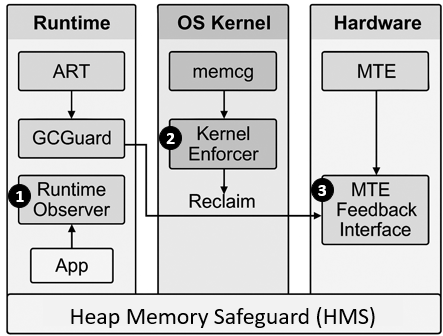
\includegraphics[width=0.85\linewidth]{./fig1_hms_architecture.png}
  \caption{Proposed HMS integration boundary.  Solid components are represented by
  the simulation; dashed Android/runtime/kernel connections are design targets.}
  \Description{Three-layer HMS concept: a user-space observer combines managed,
  native, resident, and pressure telemetry; a controller computes a reclaim
  request; and an existing memory-cgroup actuator performs bounded reclaim.  The
  repository simulates these components and does not implement Android hooks.}
  \label{fig:hms_architecture}
\end{figure}

\subsection{State Model}
For application $i$ at sample $t$, HMS records managed allocation activity
$a_i^m(t)$, sampled native allocation activity $a_i^n(t)$, RSS $R_i(t)$, the
configured memcg limit $L_i(t)$, and PSI $p_i(t)$.  The first four signals form the
controller input.  PSI is a lagging safety signal and is used to suppress additional
work during an existing severe stall, not as proof of heap ownership.

The original score is retained as an explicitly heuristic index:
\[
H_i(t)=\frac{R_i(t)}{L_i(t)}
       +\alpha\frac{\widehat{g}_i(t)}{G_i(t)} ,
\]
where $\widehat{g}_i(t)$ is an exponentially smoothed \emph{net resident-growth
estimate}, not raw object allocation, and $G_i(t)$ is an online scale.  We set
\[
G_i(t)=\max\{\epsilon,Q_{0.95}(\lvert\widehat{g}_i\rvert)
\text{ over a trailing window}\}.
\]
Only past samples enter the window; values above the current scale are clipped.
This avoids whole-experiment maxima and future-data leakage.  The score is
dimensionless, and $\alpha$ is a weight.  It is not a prediction horizon or a
calibrated time-to-pressure estimate.

For a deployable controller, a more interpretable quantity is
\[
T_i^{\mathrm{pressure}}(t)=
\frac{\max(0,L_i(t)-R_i(t))}
     {\max(\widehat{g}_i(t),\epsilon)} .
\]
The simulation retains $H_i$ to study the published lightweight policy; evaluation
of calibrated time-to-pressure error is future work.

\subsection{Control and Bounded Actuation}
Two thresholds provide hysteresis.  Crossing $\theta_1$ enters observation state;
crossing $\theta_2$ creates a reclaim request.  A request contains a cgroup
identifier, maximum byte budget, deadline class, and cooldown.  An implementation
should invoke an existing scoped actuator such as \texttt{memory.reclaim}; this
paper does not claim a \texttt{vmscan} modification, custom \texttt{GCGuard} API, or
\texttt{system\_server} service.

The budget is capped by the smaller of excess resident bytes and a per-cycle
fraction of the cgroup limit.  A cooldown prevents immediate repetition.  Refault
or rising PSI feedback reduces the next budget.  GC-active and render-deadline
windows defer reclaim unless the cgroup is at its hard limit.  These rules bound
work per cycle but do not constitute a formal stability proof.

\subsection{Concurrent Applications and Fairness}
For simultaneous requests, HMS orders foreground-deadline classes ahead of
background throughput classes and applies deficit round-robin within each class.
Each cgroup receives a token bucket proportional to its configured limit; unused
tokens carry over only to a fixed cap.  Per-cgroup and global reclaim budgets bound
one cycle.  Process exit cancels queued work, and cgroup identity must be
revalidated before actuation.  This policy prevents starvation in the model, but
priority inversion, shared-page accounting, cgroup offlining, lock contention, and
competition with direct reclaim or kswapd remain implementation questions.

\subsection{Artifact Boundary}
The Python package models telemetry, controller decisions, a memcg-like reclaim
proxy, and a tagging proxy.  It has no privileged service, Binder/eventfd path,
\texttt{heapprofd} integration, \texttt{smaps} parser, SELinux policy, or kernel
module used by the reported runs.  The historical package name \texttt{hmp} is an
import-compatibility detail.  This explicit boundary is part of the design:
simulation can test policy logic, while only a future Android implementation can
establish overhead, safety, or effectiveness on hardware.
